% This is a Basic Assignment Paper but with like Code and stuff allowed in it, there is also url, hyperlinks from contents included. 

\documentclass[11pt]{article}

% Preamble

\usepackage[margin=1in]{geometry}
\usepackage{amsfonts, amsmath, amssymb}
\usepackage{fancyhdr, float, graphicx}
\usepackage[utf8]{inputenc} % Required for inputting international characters
\usepackage[T1]{fontenc} % Output font encoding for international characters
\usepackage{fouriernc} % Use the New Century Schoolbook font
\usepackage[nottoc, notlot, notlof]{tocbibind}
\usepackage{listings}
\usepackage{xcolor}
\usepackage{blindtext}
\usepackage{hyperref}
\hypersetup{
    colorlinks=true,
    linkcolor=black,
    filecolor=magenta,      
    urlcolor=cyan,
    pdfpagemode=FullScreen,
    }

\definecolor{codegreen}{rgb}{0,0.6,0}
\definecolor{codegray}{rgb}{0.5,0.5,0.5}
\definecolor{codepurple}{rgb}{0.58,0,0.82}
\definecolor{backcolour}{rgb}{0.95,0.95,0.92}

\lstdefinestyle{mystyle}{
    backgroundcolor=\color{backcolour},   
    commentstyle=\color{codegreen},
    keywordstyle=\color{magenta},
    numberstyle=\tiny\color{codegray},
    stringstyle=\color{codepurple},
    basicstyle=\ttfamily\footnotesize,
    breakatwhitespace=false,         
    breaklines=true,                 
    captionpos=b,                    
    keepspaces=true,                 
    numbers=left,                    
    numbersep=5pt,                  
    showspaces=false,                
    showstringspaces=false,
    showtabs=false,                  
    tabsize=2
}

\lstset{style=mystyle}

% Header and Footer
\pagestyle{fancy}
\fancyhead{}
\fancyfoot{}
\fancyhead[L]{\textit{\Large{Information and Cycbersecurity - 2nd Year B. Tech}}}
%\fancyhead[R]{\textit{something}}
\fancyfoot[C]{\thepage}
\renewcommand{\footrulewidth}{1pt}



% Other Doc Editing
% \parindent 0ex
%\renewcommand{\baselinestretch}{1.5}

\begin{document}

\begin{titlepage}
    \centering

    %---------------------------NAMES-------------------------------

    \huge\textsc{
        MIT World Peace University
    }\\

    \vspace{0.75\baselineskip} % space after Uni Name

    \LARGE{
        Information and Cybersecurity\\
        Second Year B. Tech, Semester 1
    }

    \vfill % space after Sub Name

    %--------------------------TITLE-------------------------------

    \rule{\textwidth}{1.6pt}\vspace*{-\baselineskip}\vspace*{2pt}
    \rule{\textwidth}{0.6pt}
    \vspace{0.75\baselineskip} % Whitespace above the title



    \huge{\textsc{
            Intrusion Detection Systems
        }} \\



    \vspace{0.5\baselineskip} % Whitespace below the title
    \rule{\textwidth}{0.6pt}\vspace*{-\baselineskip}\vspace*{2.8pt}
    \rule{\textwidth}{1.6pt}

    \vspace{1\baselineskip} % Whitespace after the title block

    %--------------------------SUBTITLE --------------------------	

    \LARGE\textsc{
        Lab Assignment 10
    } % Subtitle or further description
    \vfill

    %--------------------------AUTHOR-------------------------------

    Prepared By
    \vspace{0.5\baselineskip} % Whitespace before the editors

    \Large{
        Krishnaraj Thadesar \\
        Cyber Security and Forensics\\
        Batch A1, PA 20
    }


    \vspace{0.5\baselineskip} % Whitespace below the editor list
    \today

\end{titlepage}


\tableofcontents
\thispagestyle{empty}
\clearpage

\setcounter{page}{1}

\section{Aim}
Configuration and demonstration of Intrusion Detection System using Snort

\section{Objectives}
To learn authentication techniques for Access Control


\section{Theory}

Host-based IDS (HIDS) and Network-based IDS (NIDS) are two types of intrusion detection systems that are used to monitor and detect potential security threats.

\subsection{HIDS - Host-based IDS}

A Host-based IDS (HIDS) is an IDS system that is installed on individual hosts or endpoints to monitor the activity on that host. It uses system logs, file integrity checks, and other methods to identify potential security threats. The HIDS can detect attacks that are not visible on the network, such as local privilege escalation, malware infections, and unauthorized access attempts.\\

Example: OSSEC is an open-source HIDS that can detect various host-based attacks, including rootkits, file changes, and unauthorized access attempts. It uses a combination of signature-based, anomaly-based, and heuristic-based detection methods to increase the accuracy of attack detection and reduce false positives.

\subsection{NIDS - Network-based IDS}

A Network-based IDS (NIDS) is an IDS system that is installed on the network to monitor traffic passing through it. It analyzes packets passing through the network to identify suspicious behavior, such as unusual traffic patterns, unauthorized access attempts, and malware infections. NIDS can detect attacks that are visible on the network, but may not detect attacks that are targeted to a specific host or endpoint.\\

Example: Snort is an open-source NIDS that can detect a wide range of attacks and anomalies in network traffic. It uses a combination of signature-based, anomaly-based, and heuristic-based detection methods to increase the accuracy of attack detection and reduce false positives. Suricata is another open-source NIDS that can detect various network-based attacks, including DDoS, malware infections, and suspicious traffic patterns.\\

HIDS and NIDS can be used together to provide a comprehensive security solution. While HIDS is good at detecting attacks on a specific host or endpoint, NIDS can detect attacks that are not visible on the host or endpoint. Using both HIDS and NIDS can help provide a layered security approach to detect and respond to potential security threats.


\begin{figure}[H]
    \centering
    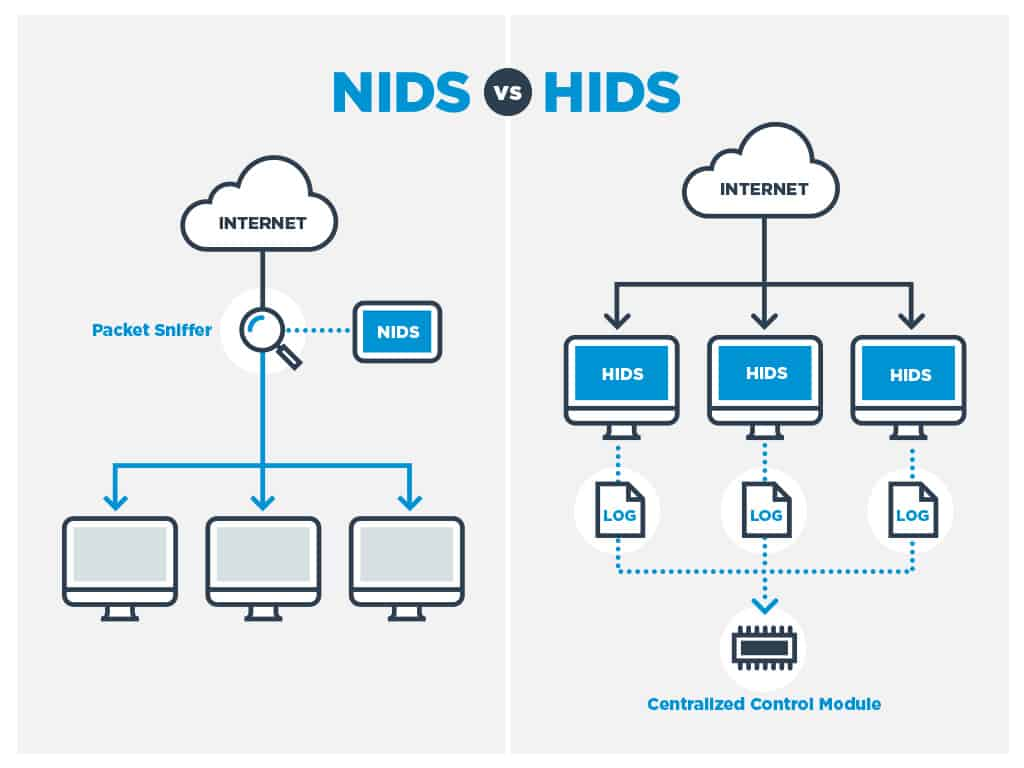
\includegraphics[width=.85\textwidth]{NIDS-vs-HIDS.jpg}
\end{figure}
\section{Platform}
\textbf{Operating System}: Arch Linux x86-64 \\
\textbf{IDEs or Text Editors Used}: Visual Studio Code\\
\textbf{Compilers or Interpreters}: Python 3.10.1\\

\section{Input and Output}

\begin{verbatim}
% The Given Signature is Valid
\end{verbatim}

% \section{Code}
% \lstinputlisting[language=Python, caption="DSA Signature Validity using PyCrypto Library"]{../Programs/Assignment_7/dsa using lib.py}

\section{Conclusion}
Thus, We have learnt IDS systems and their types. We have also learnt about various tools based on IDS systems.
\clearpage

\section{FAQ}

\begin{enumerate}
    \item \textbf{What are various types of IDS system?}\\

          There \textit{are two main types of IDS systems}:
          \begin{enumerate}
              \item \textit{Network-based IDS (NIDS)}: NIDS systems monitor network traffic in real-time to detect and alert on potential attacks. They analyze packets passing through the network to identify suspicious behavior, such as unusual traffic patterns, unauthorized access attempts, and malware infections.
              \item \textit{Host-based IDS (HIDS)}: HIDS systems monitor the activity on individual hosts to detect and alert on potential attacks. They analyze system logs, file integrity, and user activity to identify suspicious behavior, such as unauthorized access, malware infections, and changes to system configurations.
          \end{enumerate}

    \item \textbf{What are the popular tools based on IDS systems?}\\

          There \textit{are several popular tools based on IDS systems, including}:

          \begin{enumerate}
              \item \textit{Snort}: an open-source NIDS that can detect a wide range of attacks and anomalies in network traffic.
              \item \textit{Suricata}: an open-source NIDS that can detect and alert on various network-based attacks, including DDoS, malware infections, and suspicious traffic patterns.
              \item \textit{OSSEC}: an open-source HIDS that can detect and alert on various host-based attacks, including rootkits, file changes, and unauthorized access attempts.
              \item \textit{Bro}: an open-source NIDS that can detect and alert on various network-based attacks, including malware infections, network scans, and suspicious traffic patterns.
              \item \textit{Security Onion}: a Linux distribution that includes several IDS tools, including Snort, Suricata, and Bro, and provides a centralized platform for monitoring and analyzing network and host activity.
          \end{enumerate}

    \item \textbf{What are the detection methods of IDS?}\\
          IDS systems use several methods for detecting potential attacks, including:
          \begin{enumerate}
              \item \textit{Signature-based detection}: IDS systems can detect known attacks by comparing network or host activity to a database of known attack signatures. If a match is found, the IDS can generate an alert.
              \item \textit{Anomaly-based detection}: IDS systems can detect new or unknown attacks by identifying patterns or behavior that deviate from normal or expected activity. This method requires a baseline of normal activity to be established, which the IDS can then use to identify anomalies.
              \item \textit{Heuristic-based detection}: IDS systems can detect potential attacks by using algorithms and rules to identify behavior that is indicative of an attack. This method can be more flexible than signature-based detection, but can also result in more false positives.
              \item \textit{Hybrid detection}: IDS systems can use a combination of signature-based, anomaly-based, and heuristic-based detection methods to increase the accuracy of attack detection and reduce false positives.
          \end{enumerate}


\end{enumerate}

\end{document}